% !TEX root = linearpartition.tex

\setcounter{figure}{0}
\renewcommand{\thefigure}{Online Method \arabic{figure}}
\setcounter{table}{0}
\renewcommand{\thetable}{Online Method \arabic{table}}

\section*{Online Methods}

%We propose LinearFold,
%% LinearFold is 
%% a linear-time prediction algorithm predicting RNA
%% secondary structures.
% Our \linearfold approach is 
% presented in four steps, starting from
% the most naive but easy-to-understand exhaustive search version (Fig.~\ref{fig:method} C1), and gradually 
% build it up to 
% the linear-time version (Fig.~\ref{fig:method} C4), using a stack-top merge and beam search.

Here we first formulate the \linearfold algorithm more formally.

\subsection*{Formulation}
%% The RNA secondary structure prediction problem can be formalized as follows,
%% using the dot-bracket format to represent structures.
Generally, given an input RNA sequence
$$ \vecx = x_1x_2\ldots x_{n}, \text{ where } x_i \in \{\tt{A},\tt{C},\tt{G},\tt{U}\},$$
the RNA secondary structure prediction algorithm
%$\mathit{f}$ 
aims to find the best-scoring pseudoknot-free structure
%$$ \vecy = y_1y_2\ldots y_{n}, \text{ where } y_i \in \{\md, \ml, \mr\}$$
%(to address pseudoknots, different types of brackets would be required)
according to a scoring function \score (e.g., model score or negative free energy) parameterized by model $\weight$:
% (or minimum model cost):
\vspace{-0.1cm}
% \begin{equation}
%   %f(\vecx) =
%   \argmax_{\vecy \in \GEN(\vecx)} \score(\vecx, \vecy; \weight)
%   \label{eq:mfe}
% \end{equation}
%\vspace{-0.2cm}
where $\GEN(\vecx)$ is the set of all possible pseudoknot-free structures
\[
\GEN(\vecx) =
\big\{\vecy \in \{\md, \ml, \mr\}^n \;\mid\; \vecy \text{~is balanced in brackets}\big\}.
\]
%and %$\score$ is the cost function (i.e., free
%energy function), and
The two baselines in our study, \contrafold
and \viennarnafold, use scoring functions that are very similar  in structure, % scoring functions,
but very different in parameters 
(the former learns \vecw from data, % in which the free energy
%is not revealed,
while the latter is based on thermodynamics).

All dynamic programming-based prediction algorithms, including ours, %like previous ones, are based on dynamic programming,
require the scoring function to {\em decompose} to the scorings of smaller structures,
in order to have efficient computation.
For example, the main text (see Fig.~\ref{fig:method}) uses the simplest Nussinov-style scoring function 
that factors to each individual base pair and simply counts the number of pairs in a structure:
\begin{equation}
  \score_{\text{Nussinov}}(\vecx, \vecy; \_) = \# \pairs(\vecy) = \sum_{(i,j)\in \pairs (\vecy)} 1
  \label{eq:nussinov}
\end{equation}
where $\pairs(\vecy)$ returns the list of base pairs in \vecy, e.g.,
$\pairs(\text{``\md\ml\ml\md\mr\mr\md''}) = \{(2,6), (3,5)\}$.
Note this scoring function does not depend on any model,
but we could in principle assign different scores in \vecw for GC, AU, and GU pairs (e.g., $w_\text{GC} > w_\text{AU} > w_\text{GU}$),
and also introduce a penalty for each unpaired nucleotide ($w_\unpaired < 0$),
which we call the ``Extended Nussinov'' model:
\begin{equation}
  \score_{\text{extended}}(\vecx, \vecy; \vecw) = \sum_{(i,j)\in \pairs (\vecy)} w_{x_i x_j} +\sum_{i\in \unpaired(\vecy)} w_\unpaired
  \label{eq:extended}
\end{equation}
In reality, the actual scoring functions % $\score$ (scoring structure \vecy on input \vecx by model \vecw) can be
used by \contrafold, \rnafold, and \linearfold are more complex and they
decompose to individual loops: % as follows:
\begin{equation}
  \begin{split}
 \score_\text{real}(\vecx, \vecy; \weight) = &
 \!\!\!\!\sum_{h \in \text{hairpin\_loops}(\vecy)}\!\!\!\! \score^{\mathrm H}(\vecx, h; \weight)  + \!\!\!\!\sum_{s \in \text{single\_loops}(\vecy)}\!\!\!\! \score^{\mathrm S}(\vecx, s; \weight) \\
 + & \!\!\!\!\sum_{m \in \text{multi\_loops}(\vecy)}\!\!\!\! \score^{\mathrm M}(\vecx, m; \weight) +  \!\!\!\!\sum_{e \in \text{external\_loops}(\vecy)}\!\!\!\!\!\!\!\! \score^{\mathrm E}(\vecx, e; \weight).
\end{split}
\label{eq:decomp}
\end{equation}
The thermodynamic %minimal free energy
model in \viennarna scores %, the score of constructing 
each type of loop %(hairpin, single-branch, multi-branch, and external)
using several feature templates such as
hairpin/bulge/internal loop lengths,
terminal mismatches, helix stacking, helix closing, etc.
%% %the following feature components:\cite{mathews+:1999}
%% \begin{itemize}[itemsep=-1mm]
%% \item %$\score^{\mathrm H}(\cdot,\cdot;\cdot)$,
%% Hairpin loops: hairpin length, terminal mismatch, and special tri-, tetra-, and hexa-loops. 
%% \item %$\score^{\mathrm S}(\cdot,\cdot;\cdot)$,
%% Single-branch loops (including helix stacking as empty loop, and bulge and internal loops):
%% bulge length, internal loop length, internal loop left-right balancing,
%% terminal mismatch, helix stacking, and helix closing.
%% \item %$\score^{\mathrm M}(\cdot,\cdot;\cdot)$,
%% Multi-branch loops: multi-loop base cost, terminal mismatch,
%% left/right dangles, multi paired, and multi unpaired.
%% \item %$\score^{\mathrm E}(\cdot,\cdot;\cdot)$,
%% External loops: left/right dangles, external paired and external  unpaired. 
%% \end{itemize}
The machine-learned model in \contrafold
replaces energies in the above framework with model weights learned from data.
%all the model weights are learned from data, instead of the free energy.
%% We conclude
%% the cost decomposition in Fig.~\ref{fig:realdeduct}. 

%% RNA secondary structure prediction is regarded as a challenging problem,
%% that no existing model can score perfectly to match the actual
%% structure with the minimum free energy (or minimum model cost) function, i.e.,
%% {\bf imperfect modeling}.
%% Consider $y^*(\vecx)$ as the actual secondary structure of the given sequence,
%% and an evaluation metric (e.g., PPV, sensitivity) $M$ to
%% calculate accuracy of a set of predicted structures against the actual
%% structures ($M(y,y)=1$), we are likely to have $M(f(\vecx), y^*(\vecx)) < 1$
%% according to the existing results reported(see Fig.\ref{fig:accuracy}).

%% Our proposed \linearfold algorithm can linearize any system with a variant of
%% $(\score,\weight)$, as long as $f(\vecx) = \argmin_{\vecy \in \GEN(\vecx)}
%% \score(\vecx, \vecy; \weight)$ can be 
%% solved in cubic-time by the dynamic programming algorithm.
%% The linearization maintains the same cost function and model $(\score,\weight)$,
%% but the objective function is different, i.e. $f' \neq f$, as we set a series of
%% soft constraints
%% during the beam search, pruning out structures with high cost or high free
%% energy which depends on the given $(\score,\weight)$.
%% Experimental results show that
%% this difference leads to a higher accuracy in linearizing \contrafold and
%% Vienna RNAfold (see Fig.~\ref{fig:accuracy} and Fig.~\ref{fig:beamsize}).

Our \linearfold algorithm can ``linearize'' any cubic-time prediction system
as long as the scoring function decomposes in a way similar to Eqs.~\ref{eq:nussinov}--\ref{eq:decomp} above.
Below we formalize our \linearfold algorithm step by step, % as follows.
using the Extended Nussinov model in Eq.~\ref{eq:extended} to strike a balance between simplicity
and reality.
We will refer to both the high-level illustration in Fig.~\ref{fig:method},
and a more formal deductive system in Fig.~\ref{fig:deduction}.

% The basic idea of our proposed

% We propose \linearfold, the first global linear-time RNA secondary structure
% prediction algorithm. 
% The basic idea of linear-time prediction is to predict incrementally from
% left to right,
% %, inspired by human sentence processing. To adapt it to RNA
% %sequences, 
% %we view the problem as incrementally converting the RNA sequence into
% %the dot-bracket format, such that 
% labeling each nucleotide  as unpaired ``{\textbf .}'', opening ``{\textbf (}'',
% or closing ``{\textbf )}''. 
% %% This makes the
% %% dot-bracket format equivalent to the pseudoknot-free RNA secondary structures
% We require this dot-bracket string to be well-balanced as we only consider pseudoknot-free structures
% (to address pseudoknots, different types of brackets would be required. This is left as our future work). 

% the term "exponentially traverse" is strange, I suggest "traverse all possible
% structures in GEN(\vecx), which takes exponenential time
%% 4-step method claim
%\vspace{.25cm}
\subsection*{Naive exhaustive incremental prediction: $O(3^n)$ time}
By exhaustively predicting $y$ from left-to-right, we
traverse all the possible structures in $\GEN(\vecx)$,
% calculate the free energy for each of them,
and pick the one with the highest score (or lowest free energy). % or model cost.
We denote each {\em state} at step $j$ ($j \in \{0,\ldots, n\}$)
as a tuple along with a score $s$:
%\begin{equation}
\[
        \nnitem{\vecy}{\sigma}{j}{s},
\]
%$s = \nitem{{\bm \sigma} | i}{j}\vecy$,
%\end{equation}
where \vecy is the (sub)structure for the prefix $x_1 \ldots x_j$,
and
$\sigma$ is the  stack consisting of unmatched opening bracket positions in \vecy.
For the Nussinov model, score $s$ is simply the number of pairs in \vecy.
For example, if \vecy=``\md\ml\ml\md\mr\ml'', then $\sigma=[2,6]$ and $s=1$.
%and $s$ is the score of the state.
%% so far
%% where $i$ is the top of the stack, meaning $x_i$ is the last unmatched opening nucleotide. 
%$\vecy$ is the corresponding dot-bracket (sub)sequence up to $x_{j-1}$.
Each state can transition into a subsequent state, taking one of the three
actions:
\begin{enumerate}
\itemsep-0.2em
\item \push:
$\nnitem{\vecy}{\sigma}{j}{s} \goesto \nnitem{\vecy\!\circ\!{\text `}\ml{\text '}}{\sigma | j}{j+1}{s}$.
%which labels the current nucleotide $x_j$ as a left bracket ``{\textbf (}'', 
%putting it on top of the stack;
\item \nskip:
$\nnitem{\vecy}{\sigma}{j}{s} \goesto \nnitem{\vecy\!\circ\!{\text `}\md{\text '}}{\sigma}{j+1}{s + w_\unpaired}$.
%, which labels $x_j$ as a dot ``{\textbf .}'', leaving the stack unchanged,
%and 
\item \pop:
$\nnitem{\vecy}{\sigma | i}{j}{s} \goesto \nnitem{\vecy\!\circ\!{\text `}\mr{\text '}}{\sigma}{j+1}{s+ w_{x_i, x_j}}$
(if $x_i$ and $x_j$ can form a base pair).
%, which labels $x_j$ as a right bracket ``{\textbf )}'', 
%if it matches $x_i$
%nucleotide with $x_{\TOP}$, the top of the stack, 
%and popping $i$ from the stack.
\end{enumerate}
See Fig.~\ref{fig:deduction}(a) for the deductive system.
% labeled dot-bracket sequences ($|y|=j$).
% Then the prediction algorithm
% starts with \(\nitem{\sigma_{\epsilon}}{0}{\epsilon}\), and ends with
% $|\GEN(x)|$ different states,
% \begin{equation}
%   \nitem{\sigma_{\epsilon}}{n}{y} ,y \in \GEN(x).
% \end{equation}
%% Starting at the state \(\nitem{\sigma_{\epsilon}}{0}{\epsilon}\), it takes
This algorithm takes $O(3^n)$ time to exhaustively traverse all possible
%structures (see the first part of Figure~\ref{fig:method}).
structures (see Figure~\ref{fig:method}D1).

% we start with an empty structure, with the current
% index at the beginning of the sequence, 
% The algorithm is
% with $O(3^n)$ time. 

% the structure $y \in \GEN(x)$ satisfies $y =y_1y_2...y_n, y_i \in \{\textbf{. (
%   )}\}$, with a balanced of brackets. We note $\pair(y) = \{(i,j) | (y_i,y_j)
% \text{~matches~in~brackets}\}$. 

% Now, given an free energy function
% $\energy$ and a model $\weight$ , our algorithm is to find the structure with
% the minimum free energy,

% we view the problem as incrementally converting the RNA sequence into the
% dot-bracket format, that each nucleotide can be labeled as unpaired ``{\tt .}'' (a
% skip action), opening ``{\tt (}'' (a push action), or closing ``{\tt )}'' (a pop
% action). The naive exhaustive prediction method would seem to require $O(3^n)$
% time, as there are 3 different labels for each nucleotide.

%\vspace{.25cm}
\subsection*{Dynamic Programming via Identical-Stack Merging:
  $O(2^{n})$ time}

Now we apply dynamic programming on top of this exhaustive method to exploit
shared computations.
Consider a simple case that two states can be merged: if
there are two states in the same step $j$,
% $\nitem{\bm \sigma}{j}\vecy$ and $\nitem{\bm \sigma}{j}{\vecy'}$, 
% sharing the exact same stack $\bm \sigma$ but with different dot-bracket strings $\vecy$ and $\vecy'$, 
%i.e.,
%they have the same positions of all unpaired openings %, means that they have identical stacks, 
we say that these two states are ``equivalent'' and we can merge them
(and only keep the better scoring between \vecy and $\vecy'$). 
%A merged state can be represented as $\twotuple{\bm \sigma}{j}$. 
Fig.~\ref{fig:method}B(Idea 1)/D2 illustrates this merging and
Fig.~\ref{fig:deduction}(b) shows the deductive system. 
Although we merge to reduce the number of states, it is still exponential time, 
% use fewer states to process, the number of
% possible states are still exponential,
since there could be exponentially many
different stacks in each step. 
% against the current index $j$.
This algorithm takes $O(2^{n})$ time. 
%%  for every possible stack
%% $\twotuple{\bm \sigma}{j}$ considered in the prediction process.

%\vspace{.25cm}
\subsection*{Dynamic Programming via Stack Top Packing: $O(n^3)$ time}

To avoid considering exponentially many states, 
we further
%% further apply the
%% Graph-Structured Stack (GSS, \cite{Tomita:1988}) to the dynamic programming. 
pack states with different stacks.
Consider two states in the same step $j$,
% $\twotuple{{\bm \sigma_0} | i}{j}$ and $\twotuple{{\bm \sigma_1} | i}{j}$,
which share the last unpaired opening $i$ (i.e., stack top). 
%(where $i$ is the same top of the stack).
We call these states ``temporarily equivalent'', since they can be treated as
exactly the same until the unpaired opening $x_i$ is closed (and thus popped from the stack).
% In other words we can represent both stacks ${\bm \sigma_0} | i $ and ${\bm \sigma_1} | i$
as $...i$, where $...$ denotes part of the history that we do not need at this moment.
This factorization of stacks is called ``Graph-Structured Stacks'' (GSS) by Tomita. \cite{Tomita:1988}
After packing, we define the new state to be $\tuple{i,j}$
%In our dynamic programming prediction algorithm, 
and therefore we  maintain $O(n^2)$ states.
For each state $\tuple{i,j}$, the pop action
can take worst-case $O(n)$ time because $\tuple{i,j}$ can combine with every $\tuple{k,i}$ from step $i$.
%due to the graph-structured stack. 
Thus the overall time complexity is $O(n^3)$.
See Fig.~\ref{fig:method}B(Idea 2)/D3 for  
an example of the packing process
and Fig.~\ref{fig:deduction}(c,d)
for the deductive system.

Now we explain the
packing on these ``temporarily equivalent'' states in detail. 
We use the GSS \cite{Tomita:1988} to pack and unpack
them, which has been widely used in parsing natural language sentences.
\cite{huang+sagae:2010}
% The idea is to combine
The idea behind the packing process is to combine the left structure information
of different states packed together in the push action,
and this structure is later unpacked in the future pop action.

Basically, if state $r$ generates state $s$ by a push action, then $r$ is added
onto $\pi(s)$, a set of predictor states. When two equivalent pushed states get
packed, we combine their predictor states. For example, if $r_x =
\tuple{t_x, j}$ predicts $s = \tuple{j,j+1}$ for $x\in \{0,\ldots, k\}$, then $\pi(s) =
\{r_x|x=0 \ldots k\}$. 
% In the pop step, state $s = \tuple{i,j}$ tries to combine with every predictor
% state $r \in \pi(s)$, and the resulting state $t$ inherits the predictor states
% set from $r$, i.e., $\pi(t) = \pi(r)$. 
To pop state $s = \tuple{i,j}$, we combine it with each of its predictor states
$r \in \pi(s)$ to make a resulting state $t$.
$t$ inherits the predictor states from $r$, i.e., $\pi(t) = \pi(r)$.

% We further merge them together since they can be treated as
% exactly same state until the unpaired opening $i$ has
% been closed. In other words, these two states are ``temporarily equivalent''.
% Although they are not equivalent states, comparing to the full-stack merge, the
% computation of these two states are with no difference before the last unpaired
% openings has been closed.
% An example of the merged prediction process is shown in Figure~\ref{fig:method}. 

Moreover, the empirical running time of our algorithm is better than cubic.
As we restrict only three types of allowed pairs ({\tt AU}, {\tt CG},
{\tt GU}) in the prediction, the pop action happens only if $(x_i, x_{j+1})$ is
one of the allowed pairs. Thus, in the skip action, we can skip nucleotides
until the next one $x_{j+1}$ can be paired with $x_i$.
We observe this emperical running time is approximately $O(n^{2.6})$, similar to
previous bottom-up dynamic programming methods.\cite{do+:2006,
  lorenz+:2011, mathews+turner:2006}

%% Similar to previous methods, we avoid sharp turns as well. All base-pairs in the
%% predicted RNA secondary structures must be with a distance $\geq 4$. 

% There is a no-sharp-turn setting in the previous methods as well, that all
% base-pairs in the predicted RNA secondary structure must be with a distance
% $\geq 4$ nucleotides, so that sharp turns in the RNA secondary structure are
% avoided.

%\vspace{.25cm}
\subsection*{Dynamic Programming via Beam Search: $O(n)$ time}
Although our stack-top packing version still runs cubically, the same as the
conventional baselines, 
 this left-to-right search is easily ``linearizable'' 
unlike the bottom-up CKY-based algorithms used by most of the existing systems for RNA structure prediction.
%, especially with long sequences.
% with a rich feature set in the RNA secondary structure prediction
% problem.
We further employ beam search pruning \cite{huang+:2012} 
to reduce the complexity to linear time.
% Thus we extend it with a beam search framework.
%% need or not?
% Although our dynamic programming algorithm is the of same complexity as 
% traditional algorithms, the key difference is that our new dynamic programming
% algorithm is {\bf incremental} (i.e., left-to-right) instead of  {\bf
%   bottom-up} as in traditional CKY-style algorithms (Nussinov, Zuker, McCaskill,
% etc.), which makes the beam search framework only applicable to our prediction algorithm.
Generally, we only keep the $b$ top-scoring (low-energy) states $\tuple{i, j}$ 
%by score 
for each step $j$. In this way all the lower-scoring (high-energy) states are pruned
out, and if a
structure survives to the end, it must have been one of the top $b$
states in every step.
This pruning also means that in a pop action, a state $(i,j)$ can combine with at most $b$ states $(k,i)$ from step $i$.
Thus the overall time complexity is $O(nb^2)$.
%% , i.e., a pop
%% action can produce at most $b$ subsequent states.
However, instead of generating $b^2$ new states from a pop action, % from a step $j$, 
we use \textbf{cube pruning} \cite{huang+chiang:2007} to generate the best
$b$ states, which would take $O(b\log b)$ time.
Thus the overall running time over a length-$n$ sequence is $O(nb\log b)$, see 
See Figure~\ref{fig:method}C(Idea 3)/D4 for beam search.

% Generally,
%at each step, we choose the best $b$ resulting states from all the
%merged states in this step, and use these states only for the next steps. For
% for all the merged states $\tuple{i, j}$ sharing the same $j$,
% we cut to top $b$ by their scores so far.

% Moreover, we can further improve the time complexity of the pop actions, by
% considering all of them at once using \textbf{cube
%   pruning}\cite{huang+chiang:2007}. 
% % the time complexity of the pop actions could be further improved.
% Assume we have $b$ states in step $j$, each which contain at most $b$ left
% pointers. 
% Instead of generating $b^2$ new states from their pop actions,
% We use cube pruning to generate the best
% $b$ states. This would take $O(b\log(b))$ time. 

 
% $b'$ of them can lead to a pop action
% towards the next step $j+1$, and each of them contains $b$ left pointers. 

% In the pop action of the GSS, 

% Moreover, for each step, 

% since $b$ states are maintained in each step, our pop action, 


% This beam pruning guarantees our algorithm costs a constant amount of time at
% each step, thus our prediction algorithm is linear-time overall.

% As a result, it is fairly easy to apply beam search pruning (a common search technique
% in Artificial Intelligence, see for example \cite{zhang+clark:2008}) 
   %    on top of our left-to-right algoithm,
% where we allow at most $b$ top-scoring states to survive in each step
% ($b$ is a constant called ``beam width'').
% Those lower-scoring states that do not make the cut are deemed unpromising,
% and it is unlikely (though possible) that those pruned states 
% would lead to the best result in the end.
% So beam search reduces the runtime to $O(n)$ at the cost of minor search errors.
% By contrast, applying the same pruning idea to the traditional bottom-up algorithm
% will still result in $O(n^3)$ time because the pruning here is per $[i,j]$ span 
% instead of per step $j$.

\iffalse
\subsection*{Incorporating Models}
"To directly compare our approach with previous work, \linearfoldv is
based on the thermodynamic \viennarnafold model \cite{lorenz+:2011} and uses all
of the exact same features. Similarly, 
  \linearfoldc is based on the machine learned \contrafold model \cite{do+:2006}
with all of its same features. This is so that without beam search, {\em
  LinearFold} will produce exactly the same predictions. 

We also observe the difference between these two types of models. More details
are provided in the Supplementary Information (SI). 
\fi

%\vspace{.25cm}
\subsection*{Dataset, Evaluation Metrics and Significance Testing}\label{dataset}
We choose the ArchiveII dataset, \cite{sloma+mathews:2016}
a diverse set of over 3,000 RNA sequences with known secondary structures.
But since the current \contrafold machine-learned model (v2.02) is trained on the S-Processed dataset \cite{andronescu+:2007}
%\footnote{\url{http://www.rnasoft.ca/CG/}}, 
we removed those sequences that appeared in the S-Processed dataset. 
The resulting dataset we used contains 2,889 sequences over 9 families, with an average length of 222.2 \nts. 

We use a sampled subset of RNAcentral to test our efficiency and scalability
performance. For the sampling, we evenly split the range from $1,000$ to
$244,296~$(the longest sequence) into 30 bins by log-scale, and for each bin we
randomly select up to $10$ sequences from the original data (there are bins with
$0$ or $1$ sequence only).
For each bin, we take the average over all sequences
and report the averaged time and memory cost. 

% from the ArchiveII dataset that are also found in the S-Processed set
% to have a clear separation between training and testing sets.
% Following \cite{sloma+mathews:2016}, we also removed the Group II Intron family.
%% the RNA sequences in the Mathews dataset that shares with the
%% S-Processed dataset.
%% We've also removed the Group II Intron family, according to the dataset
%% author.?

Due to the uncertainty of base-pair matches existing in comparative analysis
and the fact that there is fluctuation in base pairing at equilibrium,
we
consider a base pair to be correctly predicted if it is also displaced by one
nucleotide on a strand.\cite{sloma+mathews:2016}
Generally, if a pair $(i,j)$ is in the predicted structure, we consider it a
correct prediction if one of $(i,j)$, $(i-1,j)$, $(i+1,j)$, $(i,j-1)$, $(i,j+1)$ is in the
ground truth structure.
We also report the accuracy using exact base pair matching instead of this
method, in Figure~\ref{tab:accuracy_nos}. 
%To evaluate the accuracy, 
Both sensitivity and PPV are reported.
%Positive Predictive Value
%(PPV), 
Generally, if $\vecy$ is the predicted structure and $\vecy*$ is the ground
truth, we have
$$ \sens = \frac{\text{true positives}}{\text{true positives} +
  \text{false negatives}} =
\frac{|\vecy \cap \vecy^*|}{|\vecy^*|},$$
$$\ppv = \frac{\text{true positives}}{\text{true positives} +
  \text{false positives}} = \frac{|\vecy \cap \vecy^*|}{|\vecy|}. $$
For the statistical significance test, 
we use the paired two-tailed $t$-test to check the statistical significance,
with the type I error rate set to $0.05$,
consistent with the previous methods. \cite{xu+:2011}
%% \cite{sloma+mathews:2016}. 



\begin{figure*}[b]
\center
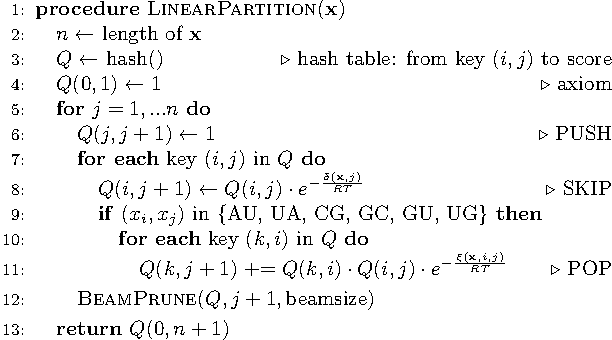
\includegraphics[scale=1]{figs/algorithm}
\caption{
LinearPartition algorithm.
\label{algorithm}}
\vspace{-0.3cm}
\end{figure*}